%! TeX root = main.tex

\documentclass[aspectratio=169]{beamer} 

\usepackage[utf8]{inputenc}
\usepackage[T1]{fontenc}
\usepackage{amsmath}
\usepackage{amssymb}
\usepackage{amsfonts}
\usepackage{mathpazo}
\usepackage{tikz}
\usepackage{parskip}
\usepackage{enumitem}
\setlist[itemize]{label=\textbullet}
\usepackage{multicol}
% \usepackage{sagetex}
% \usepackage{fancyhdr}
% \usepackage[onehalfspacing]{setspace}
% \usepackage{algorithm2e}
\usepackage{listings}
\usepackage{xcolor}
\usepackage{luacolor} % Required to use the lua-ul \highLight command 
\usepackage{lua-ul}
\usepackage{minted}
\usemintedstyle{perldoc}
\usepackage[
backend=biber,
style=ieee,
sorting=ynt
]{biblatex}
\addbibresource{library.bib}

\definecolor{LightGray}{gray}{0.9}

\LuaULSetHighLightColor{LightGray}
\usepackage{hyperref} % Needs to be the last package loaded
\hypersetup{
    colorlinks   = false,    % Colors links instead of ugly boxes
    urlcolor     = blue,    % Color for external hyperlinks
    linkcolor    = blue,    % Color of internal links
    citecolor    = red,     % Color of citations
    linktoc      = section  % Make only section number in TOC clickable
}

\setminted{
    breaklines=true,
    % fontsize=\small,
    bgcolor=LightGray,
    frame=single,
    linenos=false,
}

\usetheme{csubeamer}
\usecolortheme{csucolors}


\title{Riviera GPU Overview}
\author{Ben Blount}
\institute{Data Science Research Institute}
\date{July 2025}

\begin{document}
\maketitleframe

\section{Why Use GPUs?}

\subsection{Comparing GPUs and CPUs}
\begin{frame}{GPU Compute vs CPU Compute}
	\begin{itemize}
		\item GPUs are much better at highly parallelized tasks and much worse at highly serialized tasks than CPUs due to the difference in the number of cores in the architectures of CPUs and GPUs.
		      \begin{itemize}
			      \item CPUs have few very fast cores with advanced control units and access to much larger L1, L2, and L3 caches. 
            \item GPUs have hundreds or even thousands of small slower cores that operate under a Single Instruction, Multiple Data (SIMD) model so a single control unit can control many cores at once. 
		      \end{itemize}
		\item GPUs in particular excel at tasks such as machine learning and scientific computing.
	\end{itemize}
\end{frame}

\begin{frame}{GPU vs CPU Diagram}
	\begin{figure}
		\centering
		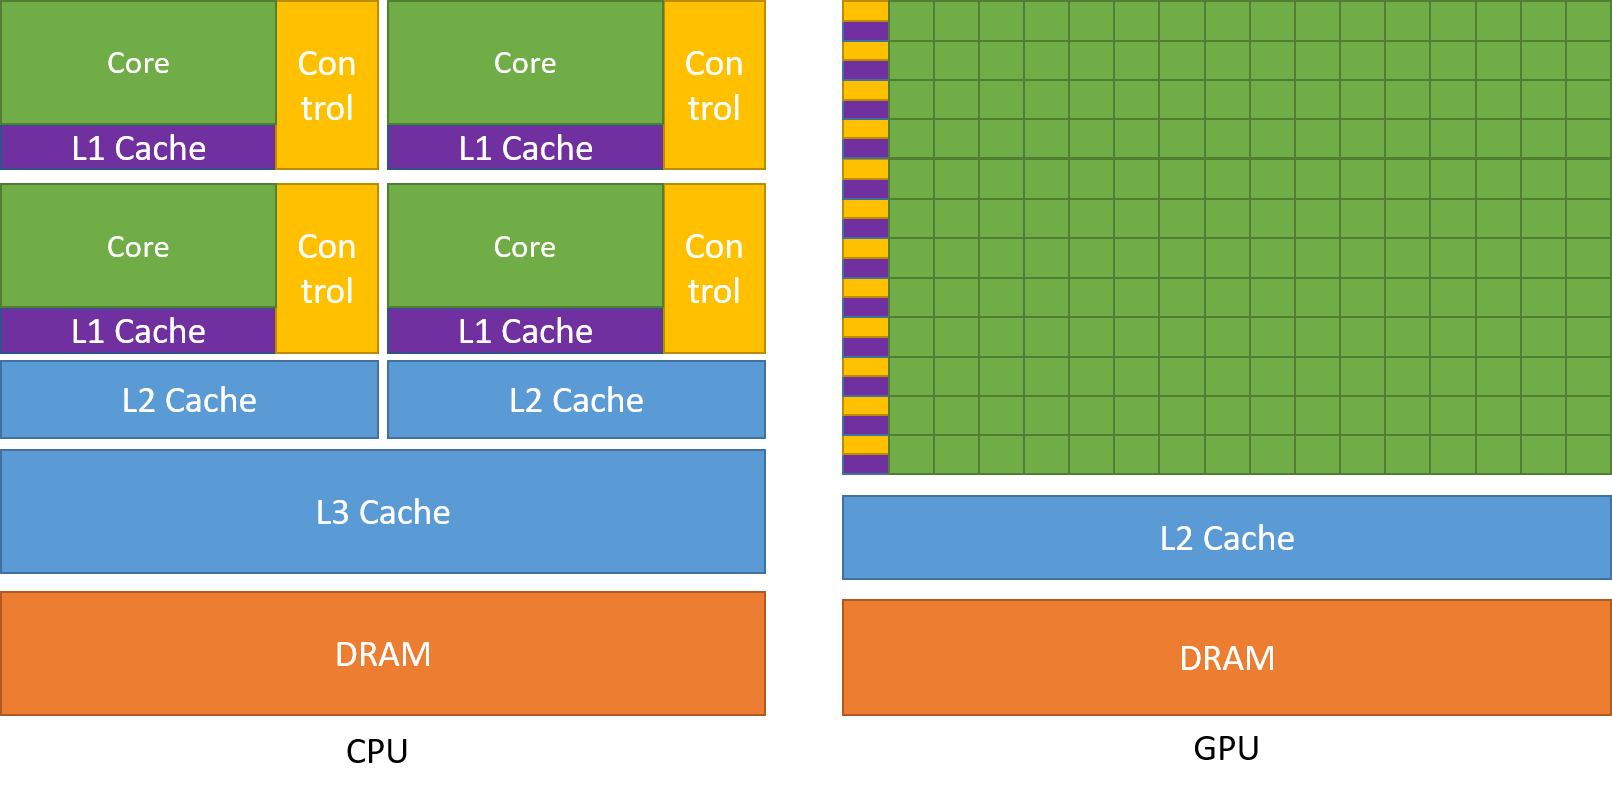
\includegraphics[scale=.4]{figures/gpu-vs-cpu.png}
    \caption{An example of CPU vs GPU core architecture from Nvidia}
	\end{figure}
\end{frame}

\subsection{A Brief Introduction to CUDA}

\begin{frame}{What is CUDA (Compute Unified Device Architecture)}
	\begin{itemize}
		\item CUDA is Nvidia's parallel computation platform and programming model that allows developers to do computation on CUDA supported GPUs.
		\item CUDA allows developers to interact directly with GPU hardware for parallelized tasks.
		\item CUDA works with a multitude of languages including C, C++, Fortran, Python, and Julia, but C++ and Python are the most common to use on Riviera.
	\end{itemize}
\end{frame}

\section{CUDA C++ Programming}
\subsection{Kernels}
\begin{frame}[fragile]{Creating Kernels}
	Kernels are functions added to C++ by CUDA that get executed \(N\) times in parallel instead of a single time serially like normal functions in C++ are. To declare a Kernel a programmer uses the \mintinline{cuda}{__global__} declaration specifier.

	\begin{minted}{Cuda}
__global__ void vector_add (float *out, float *a, float *b, int n) {
    for (int i = 0; i < n; i ++) {
        out[i] = a[i] + b[i];
    }
}
    \end{minted}

\end{frame}

\begin{frame}[fragile]{Calling Kernels}
	Once a kernel is declared, it can be called and assigned a number of threads using the \highLight{\texttt{<\vphantom{}<\vphantom{}<a,b>\vphantom{}>\vphantom{}>}} execution configuration syntax. When calling a kernel the first number \mintinline{cuda}{a} represents the number of blocks in the grid and the second number \mintinline{cuda}{b} represents the number of threads per block. This means that a total of \(a \times b\) threads are spawned organized as \mintinline{cuda}{a} blocks of \mintinline{cuda}{b} threads.

	\begin{minted}[escapeinside=||]{Cuda}
int main()
{
  ...
  VecAdd<|\vphantom|<|\vphantom|<1, N>|\vphantom|>|\vphantom|>(A, B, C)
  ...
}
  \end{minted}
\end{frame}

\subsection{Memory Management}

\begin{frame}[fragile]{Memory Management}
	When using CUDA memory has to be specifically managed on the GPU. This is achieved by allocating memory, transferring data, and deallocating memory.
	\begin{itemize}
		\item In order to allocate memory use \mintinline{cuda}{cudaMalloc(void** devPtr, size_t size)} where \mintinline{cuda}{devPtr} is a pointer to a pointer that holds the device memory address and \mintinline{cuda}{size} is the number of bytes to allocate.
		\item When copying data use \mintinline{cuda}{cudaMemcpy} which copies data from the \mintinline{cuda}{src} pointer to the \mintinline{cuda}{dst} pointer using the protocol in \mintinline{cuda}{kind} (CPU \rightarrow \, GPU, GPU \rightarrow \, GPU, GPU \rightarrow \, CPU).

		      \begin{minted}{Cuda}
cudaMemcpy(void* dst, const void* src, size_t count, cudaMemcpyKind kind)
			\end{minted}.
		\item In order to free memory use the \mintinline{cuda}{cudaFree(void* devPtr)}, which frees the memory at \mintinline{cuda}{devPtr}.
	\end{itemize}
\end{frame}

\begin{frame}[fragile]{Memory Management Code}
	\begin{minted}[escapeinside=||]{cuda}
float *a, *b, *out, *d_a, *d_b, *d_out;
a = (float*)malloc(sizeof(float) * N);
b = (float*)malloc(sizeof(float) * N);
out = (float*)malloc(sizeof(float) * N);
... // Assign variables and do CPU related logic
cudaMalloc((void**)&d_a, sizeof(float) * N);
cudaMalloc((void**)&d_b, sizeof(float) * N);
cudaMalloc((void**)&d_out, sizeof(float) * N);
cudaMemcpy(d_a, a, sizeof(float) * N, cudaMemcpyHostToDevice);
cudaMemcpy(d_b, b, sizeof(float) * N, cudaMemcpyHostToDevice);
vector_add<|\vphantom|<|\vphantom|<1,1>|\vphantom|>|\vphantom|>(d_out, d_a, d_b, N);
cudaMemcpy(out, d_out, sizeof(float) * N, cudaMemcpyDeviceToHost);
cudaFree(d_a); cudaFree(d_b); cudaFree(d_out);
free(a); free(b); free(out);
	\end{minted}

\end{frame}

\subsection{SBatch Script}
\begin{frame}[fragile]{Sample SBatch Script}
	\begin{minted}{bash}
#!/bin/bash -l
#SBATCH --job-name=cuda-example
#SBATCH --partition=short-gpu
#SBATCH --output=out.log
#SBATCH --error=error.log
#SBATCH --time=00:01:00
#SBATCH --ntasks=1

module load cuda12.2/toolkit/12.2.2

srun nvcc vector_add.cu -o vector_add # Compiles the CUDA C++ program.
srun time ./vector_add # Runs and times the cuda program
	\end{minted}
\end{frame}

\section{PyTorch CUDA}
\subsection{Programming}
\begin{frame}[fragile]{Using PyTorch With CUDA}
	It is also possible to make use of CUDA through PyTorch. Here is a very basic PyTorch example to add two tensors together (much like our kernel in C++). Tensors are just abstractions of scalars, vectors, and matrices, where a scalar is a 0D tensor, a vector is a 1D tensor, and a matrix is a 2D tensor.

	\begin{minted}{python}
import torch
device = torch.device(torch.accelerator.current_accelerator())
# Generates 2 1D PyTorch Tensors
a = torch.randn(10_000_000, device=device, dtype=torch.float32)
b = torch.randn(10_000_000, device=device, dtype=torch.float32)
c = a + b # The vector addition
print(f"PyTorch device: {device}")
print(f"Result shape: {c.shape}")
print(f"First five elements: {c[:5]}")
	\end{minted}
\end{frame}

\subsection{SBatch Script}

\begin{frame}[fragile]{Sample SBatch Script}
	\begin{minted}{bash}
#!/bin/bash
#SBATCH --job-name=pytorch-cuda
#SBATCH --partition=short-gpu
#SBATCH --output=%A/out.out
#SBATCH --error=%A/err.err
#SBATCH --ntasks=1
#SBATCH --time=00:05:00

module load python39
module load cuda12.2/toolkit
source pytorch/bin/activate # Activate python virtual environment 
srun python3 pytorch-cuda.py
deactivate # Deactivate python virtual environment with PyTorch installed
	\end{minted}
\end{frame}

% \begin{frame}{References}
% 	\printbibliography[heading=bibintoc]
% \end{frame}

\end{document}
